\chapter{Klassendiagramm/statisches Analysemodell und Paketdiagramm}

\begin{figure}[ht]
	\centering
	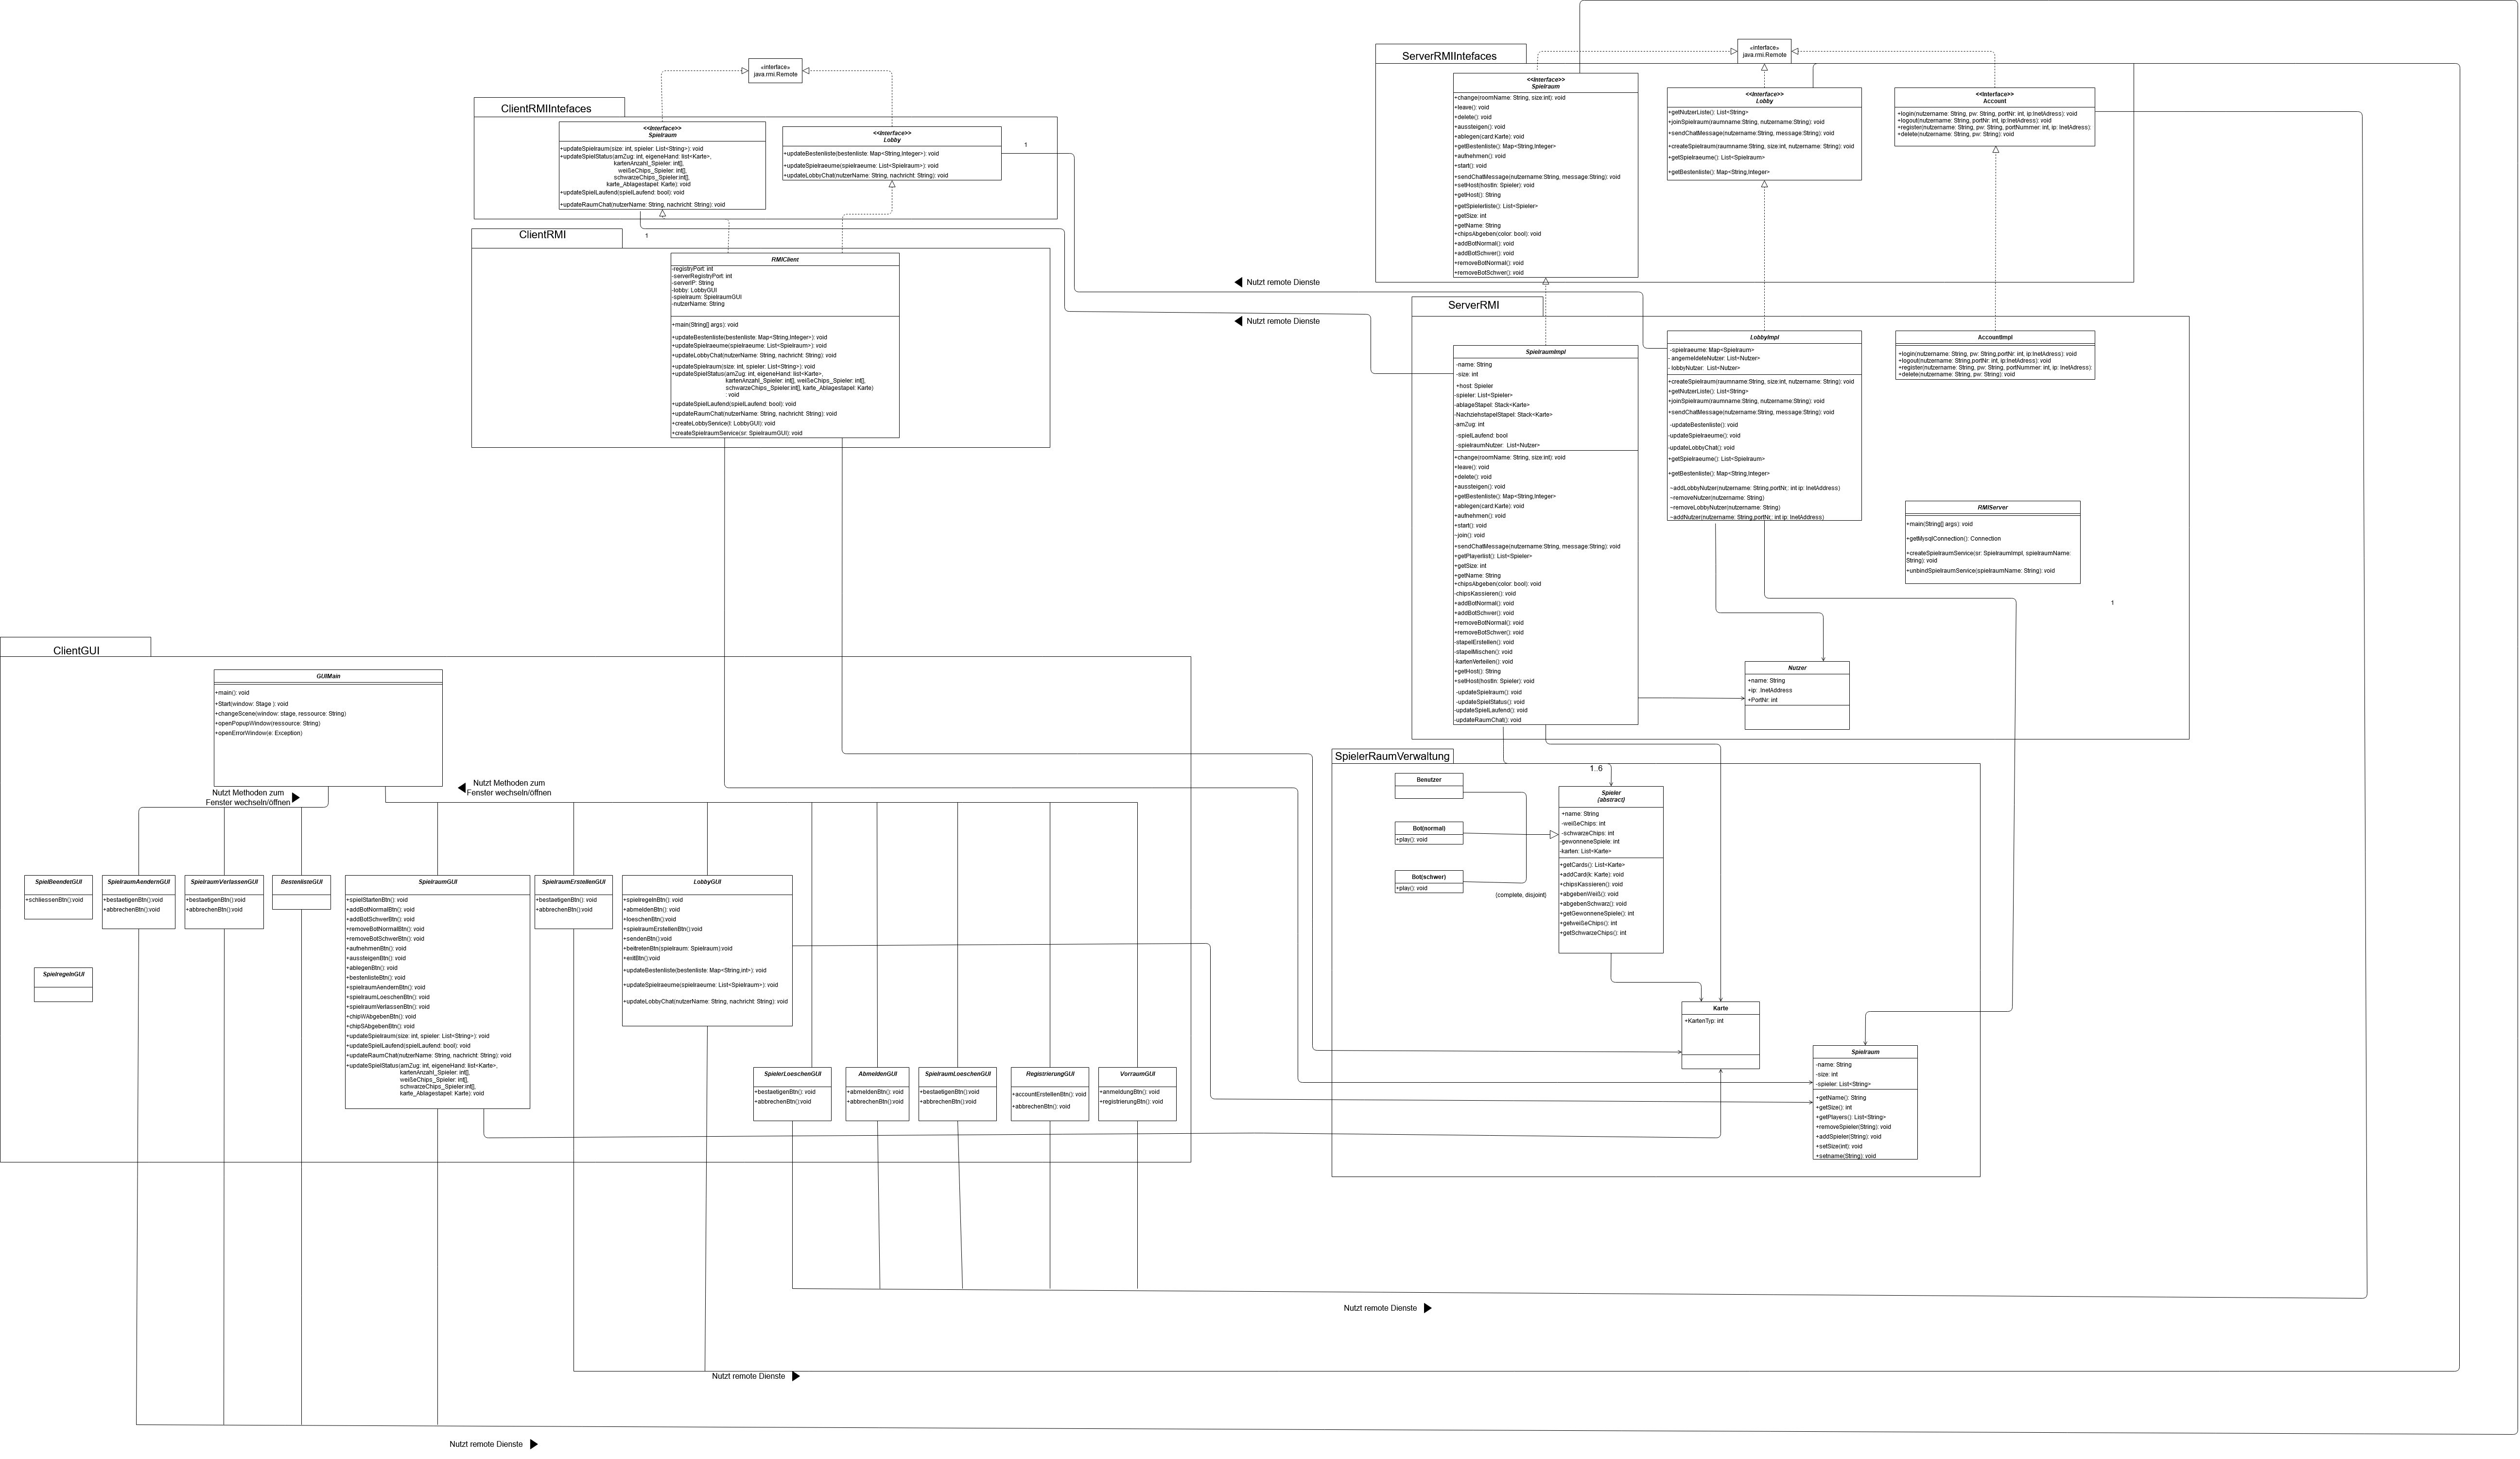
\includegraphics[height=0.9\textwidth, angle=-90]{sonstige-diagramme/Klassendiagramm.png}
	\caption{Klassendiagramm des Systems.}
\end{figure}

\begin{figure}[ht]
	\centering
	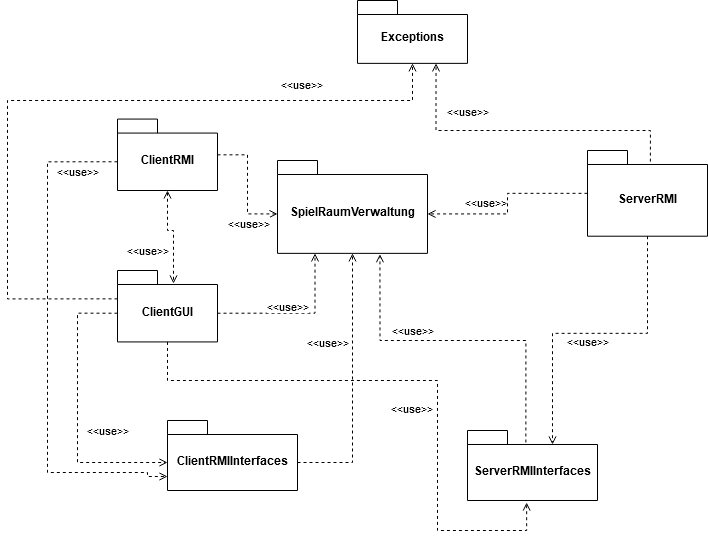
\includegraphics[width=\textwidth]{sonstige-diagramme/Paketdiagramm.png}
	\caption{Paketdiagramm des Systems.}
\end{figure}

\textbf{Anmerkungen:}\\ 
\begin{itemize}
    \item Die Attribute mit einem public modifier sind konstanten, die also nicht verändert werden können.
    \item Die Methoden in den Implementierungsklassen der Interfaces, die nicht in den Interfaces enthalten sind, dienen dem Server selbst. 
    \begin{itemize}
    \item Die private Methoden updateSpielraum, updateSpielStatus, updateSpielGestartet, updateRaumchat, updateSpielraeume und updateLobbychat werden in anderen Methoden der jeweiligen Klasse aufgerufen, um die Clients zu updaten/über die Änderungen zu informieren. Deshalb haben die Clients auch einen RMI Server und der Server speichert die IP-Adressen und Portnummern, um die Dienste zu lokalisieren. In den genannten Methoden werden die remote Methoden dieses RMI-Servers aufgerufen.
    \item Die Methoden mit dem package modifier werden in den anderen Klassen das Servers verwendet, z.B. wird join in SpielraumImpl in der Methode joinSpielraum der LobbyImpl Klasse aufgerufen, oder die Methoden addNutzer und addLobbyNutzer werden z.B. nach dem Login der Nutzer aufgerufen, um die Listen für die angemeldeten Nutzer und für die Nutzer in der Lobby zu updaten usw.
    \end{itemize}

\end{itemize}